% burndown charts
\section{Documentación}

Este trabajo práctico se realizó siguiendo la metodología ágil Scrum.
A continuación, se puede observar el gráfico Burndown correspondiente al Sprint
desarrollado para concluir las tareas necesarias para la demo final.
El mismo fue obtenido automáticamente a partir de la herramienta utilizada RallyDev.
\newline


\centerline{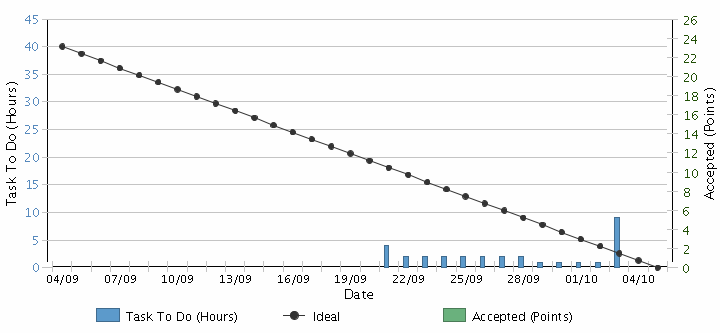
\includegraphics[width=1\textwidth]{./imagenes/burndown.png}}



A partir del gráfico, se puede notar que la mayor parte de las tareas fueron progresando
desde aproximadamente la mitad del sprint. 
También se puede notar que sobre el final del sprint se completaron las tareas.


Se puede observar en el gráfico la inconsistencia del desarrollo del proyecto. Esto ocurrió principalmente por haber agregado y eliminado
tanto stories como tareas ya estando en la etapa de desarrollo. Se debería haber definido inicialmente, sin lugar
a modificaciones, todas las especificaciones por parte del cliente y las tareas que son requeridas para cada una.
Luego de la reunión intermedia realizada con el Product Owner se agregaron nuevas tareas y se eliminaron otras,
generando así un desorden en la organización.